\documentclass[tikz, border=1mm]{standalone}

\usepackage{pgfplots}
\pgfplotsset{compat=1.15}
\usepackage{mathrsfs}
\usepackage{amsmath}
\usepackage{amssymb}
\usetikzlibrary{arrows}
\pagestyle{empty}

\usepackage{amsmath,mathrsfs}

\usetikzlibrary{matrix,positioning,fit,shapes.geometric}
\newcommand{\mydot}{\raisebox{3ex}{$\cdots$}}

\begin{document}

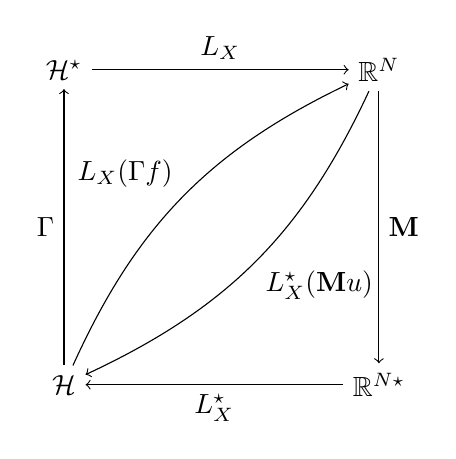
\begin{tikzpicture}


\node (H_set) at (0, 0) {$\mathcal{H}$};
\node (H_star_set) at (0, 4) {$\mathcal{H}^\star$};
\node (R_set) at (4, 4) {$\mathbb{R}^N$};
\node (R_star_set) at (4, 0) {$\mathbb{R}^{N \star}$};

\draw[->, left] (H_set) to node {$\Gamma$} (H_star_set);
\draw[->, above] (H_star_set) to node {$L_X$} (R_set);
\draw[->, right] (R_set) to node {$\mathbf{M}$} (R_star_set);
\draw[->, below] (R_star_set) to node {$L^{\star}_{X}$} (H_set);
\draw[bend left=20, ->] (H_set) to node [auto] {$L_{X}(\Gamma f)$} (R_set);
\draw[bend left=20, ->] (R_set) to node [auto] {$L^{\star}_{X}(\mathbf{M} u)$} (H_set);

\end{tikzpicture}

\end{document}